\tikzset{every node/.style={scale=0.8}}
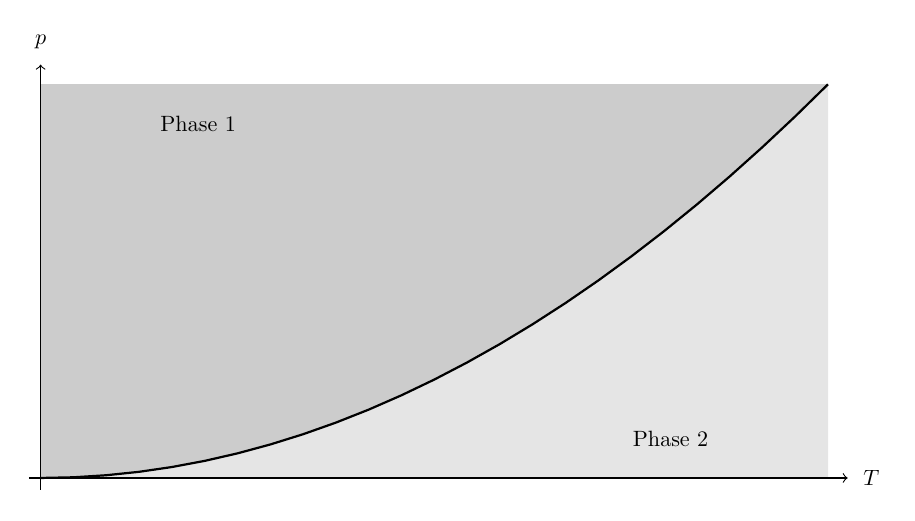
\begin{tikzpicture}[baseline=2.5cm]

  \fill[white!80!black] (0,0) rectangle (10,5);

  \fill[white!90!black,domain=0:10] (0,0) -- plot (\x,{(\x^2)/20}) -- (10,2) -- (10,0) -- cycle;


  \draw[->] (0,-0.15) to (0,5.25);
  \draw[->] (-0.15,0) to (10.25,0);
  \node[anchor=south] at (0,5.35) {$p$};
  \node[anchor=west] at (10.35,0) {$T$};

  \draw[thick,domain=0:10] plot (\x,{(\x^2)/20});

  \node at (2,4.5) {Phase $1$};
  \node at (8,0.5) {Phase $2$};

\end{tikzpicture}
